\section{Base de datos}
A continuación se describe como hemos almacenado la información extraída en la base de datos. Para una vista en detalle de las tablas véase el anexo \ref{anexo:bd}
\subsection{Noticias y municipios}
(Ver figura \ref{fig:noticias}) 
Con respecto a las noticias y pueblos almacenamos la siguiente información. Una noticia queda definida por los siguientes parámetros: Municipio al que pertenece, titular, resumen, cuerpo, fecha, dirección a la web donde se encuentra y una categoría, como información asociada a la noticia tenemos los comentarios que los usuarios pueden realizar sobre ella.

En cuanto a los municipios guardamos una serie de datos como son, nombre, provincia a la que pertenece, número de habitantes, etc. Los parámetros que definen un municipio se encuentran detallados en el capítulo \nameref{chap:obdat}. Para mostrar noticias en el caso de que no tengamos noticias de un municipio que pueda seleccionar el usuario, guardamos para cada municipio sus cinco municipios más cercanos para poder mostrar, en este caso, noticias cercanas. Además almacenamos información adicional extraída desde el Instituto de estadística y cartografía  de Andalucía\footnote{\url{http://www.juntadeandalucia.es/institutodeestadisticaycartografia}}. Para poder llevar un seguimiento de la actualización de las noticias guardamos información sobre cuando hacemos un intento de buscar nuevas noticias en los distintos municipios y saber el resultado del proceso para poder, reiniciar el proceso desde el municipio que no se pudo completar.
\section{Clasificación y categorías}
(Ver figura \ref{fig:categorias})
En la parte de clasificación guardamos la lista de categorías creadas en el capítulo \nameref{chap:categorias} que categoría o categorías se le asignan a una noticia, qué método de clasificación o usuario ha sugerido una o varias categorías para una determinada noticia, el grafo creado para la jerarquía en \ref{fig:ontologia} y las equivalencias entre las etiquetas que podemos encontrar en las páginas de los municipios y nuestras categorías.
\section{Usuarios}
(Ver figura \ref{fig:usuarios})
De los usuarios almacenamos una serie de datos básicos como un nombre de usuario y una contraseña. Por la funcionalidad que ofrece la aplicación Android, almacenamos los pueblos que quiere seguir el usuario, los comentarios que realiza y las denuncias que puede hacer sobre comentarios de otros usuarios que considere negativos, las noticias que visita y aquellas que además las valore de forma positiva y las correciones que haga sobre las categorías asignadas a una noticia.


\subsection{Control}
Las tablas que almacenan información de control son las siguientes:
\begin{center}
\centering
\begin{figure}[h]
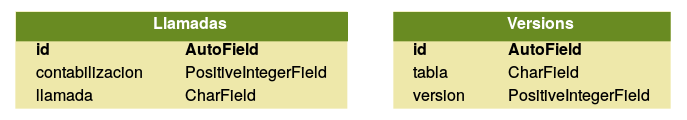
\includegraphics[scale=0.5]{basededatos/semandal_control.png}
\caption{Tablas de control}
\label{fig:control}
\end{figure}
\end{center}
En entras tablas almacenamos información estadística sobre las llamadas que se hacen a la API y las modificaciones hechas a las tablas para que desde la aplicación Android se puedan detectar estás modificaciones y actualizar algunos datos.
\begin{sidewaysfigure}
\begin{center}
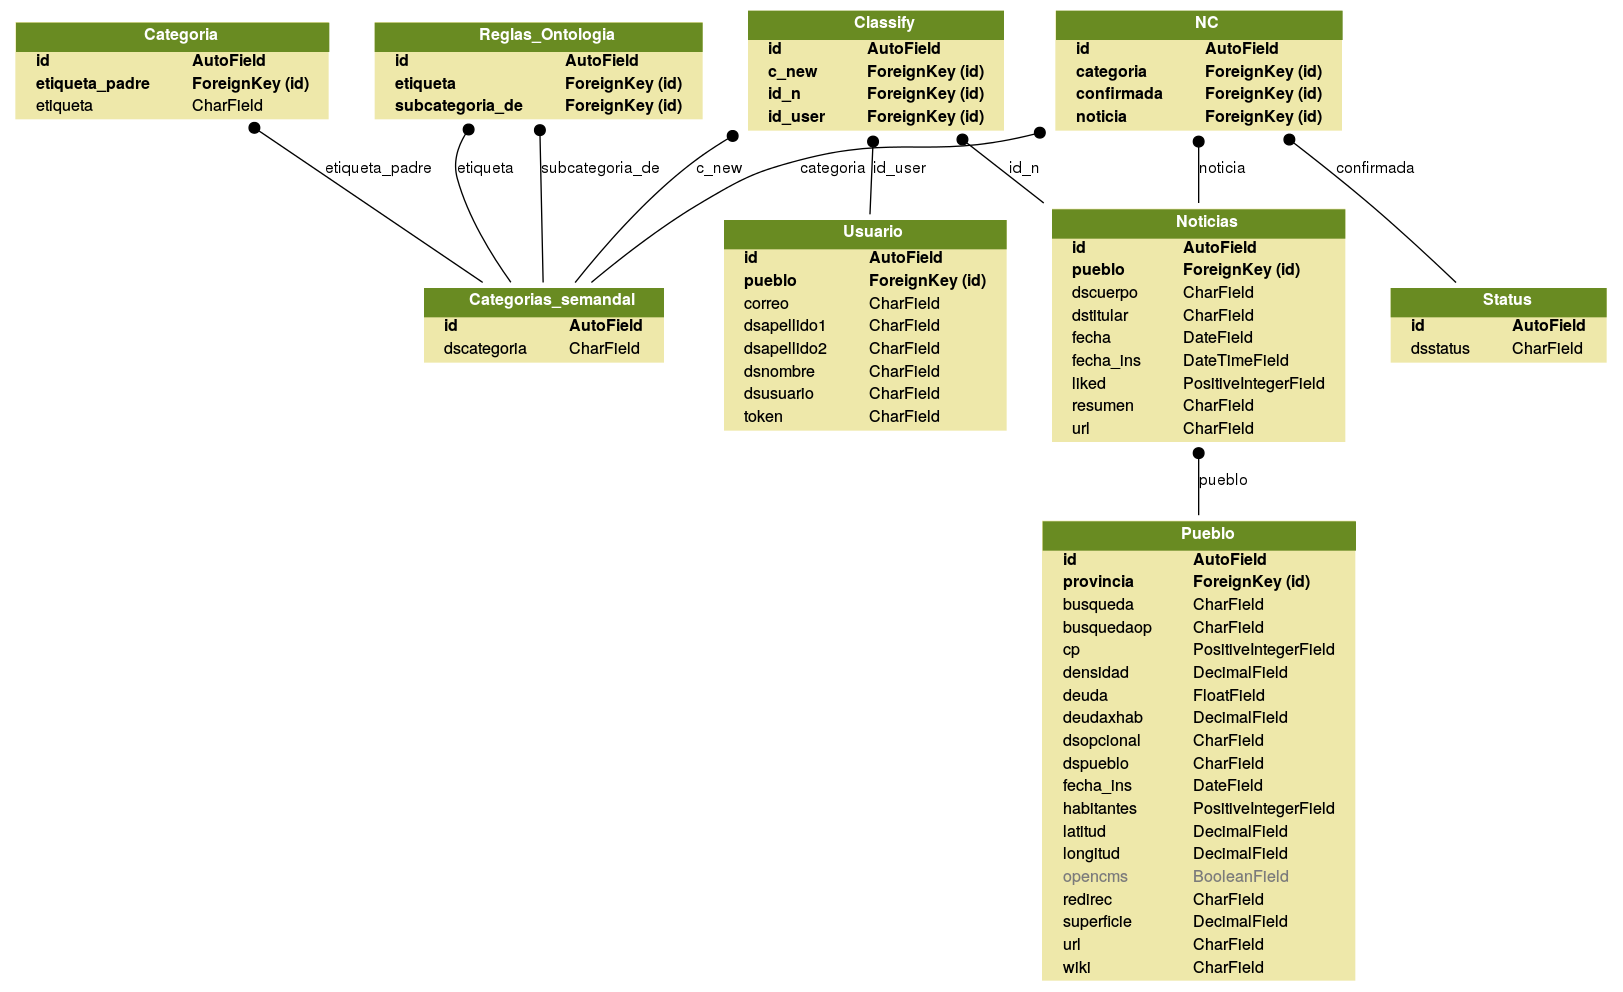
\includegraphics[scale=0.4]{basededatos/semandal_categorias2.png}
\caption{Tablas de clasificación y categorías}
\label{fig:categorias}
\end{center}
\end{sidewaysfigure}
%\subsubsection{Llamadas}
%Esta tabla almacena las distintas llamadas a la API y el número de veces que se realizan.
%\subsubsection{Versions}
%Esta tabla almacena las versiones de las tablas del proyecto para poder comprobar desde Android si se han hecho cambios y actualizar las tablas que se almacenan en el dispositivo.
\begin{sidewaysfigure}
\begin{center}
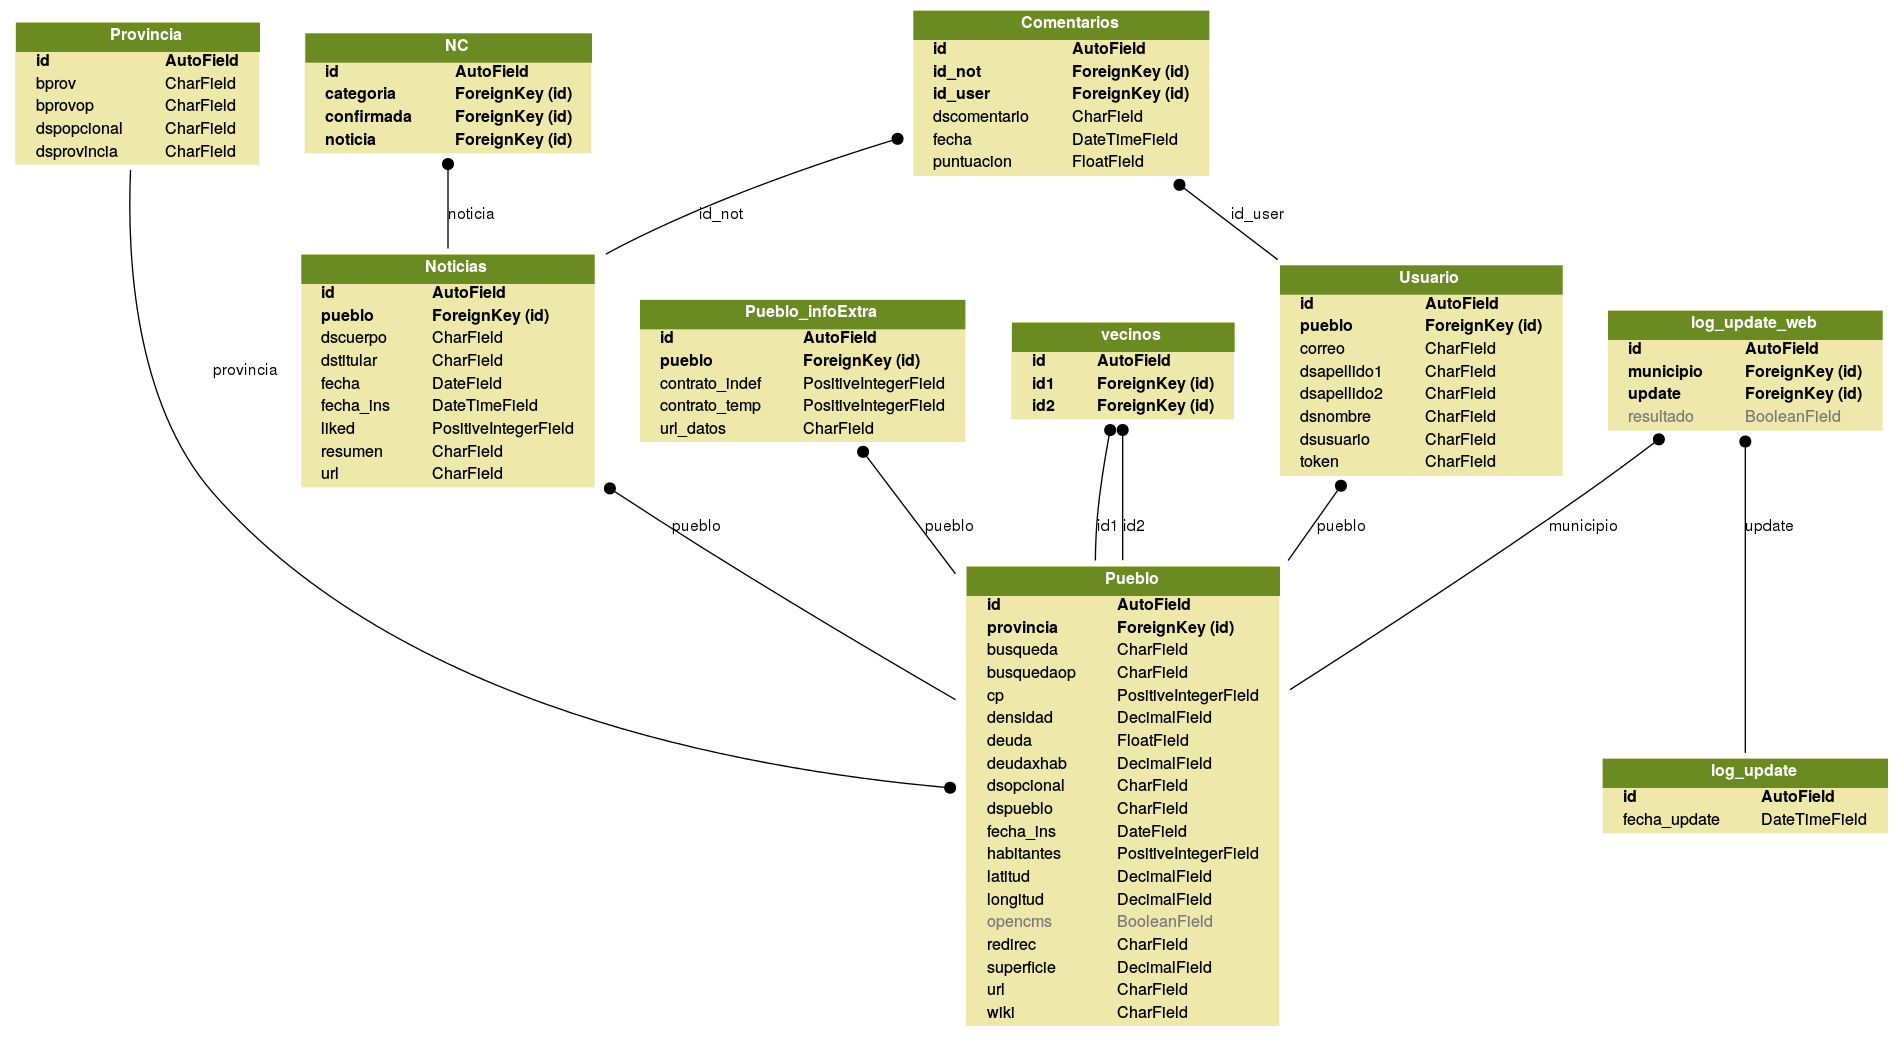
\includegraphics[scale=0.38]{basededatos/semandal_noticias2.png}
\caption{Tablas de noticias y pueblos}
\label{fig:noticias}
\end{center}
\end{sidewaysfigure}

\begin{sidewaysfigure}
\begin{center}
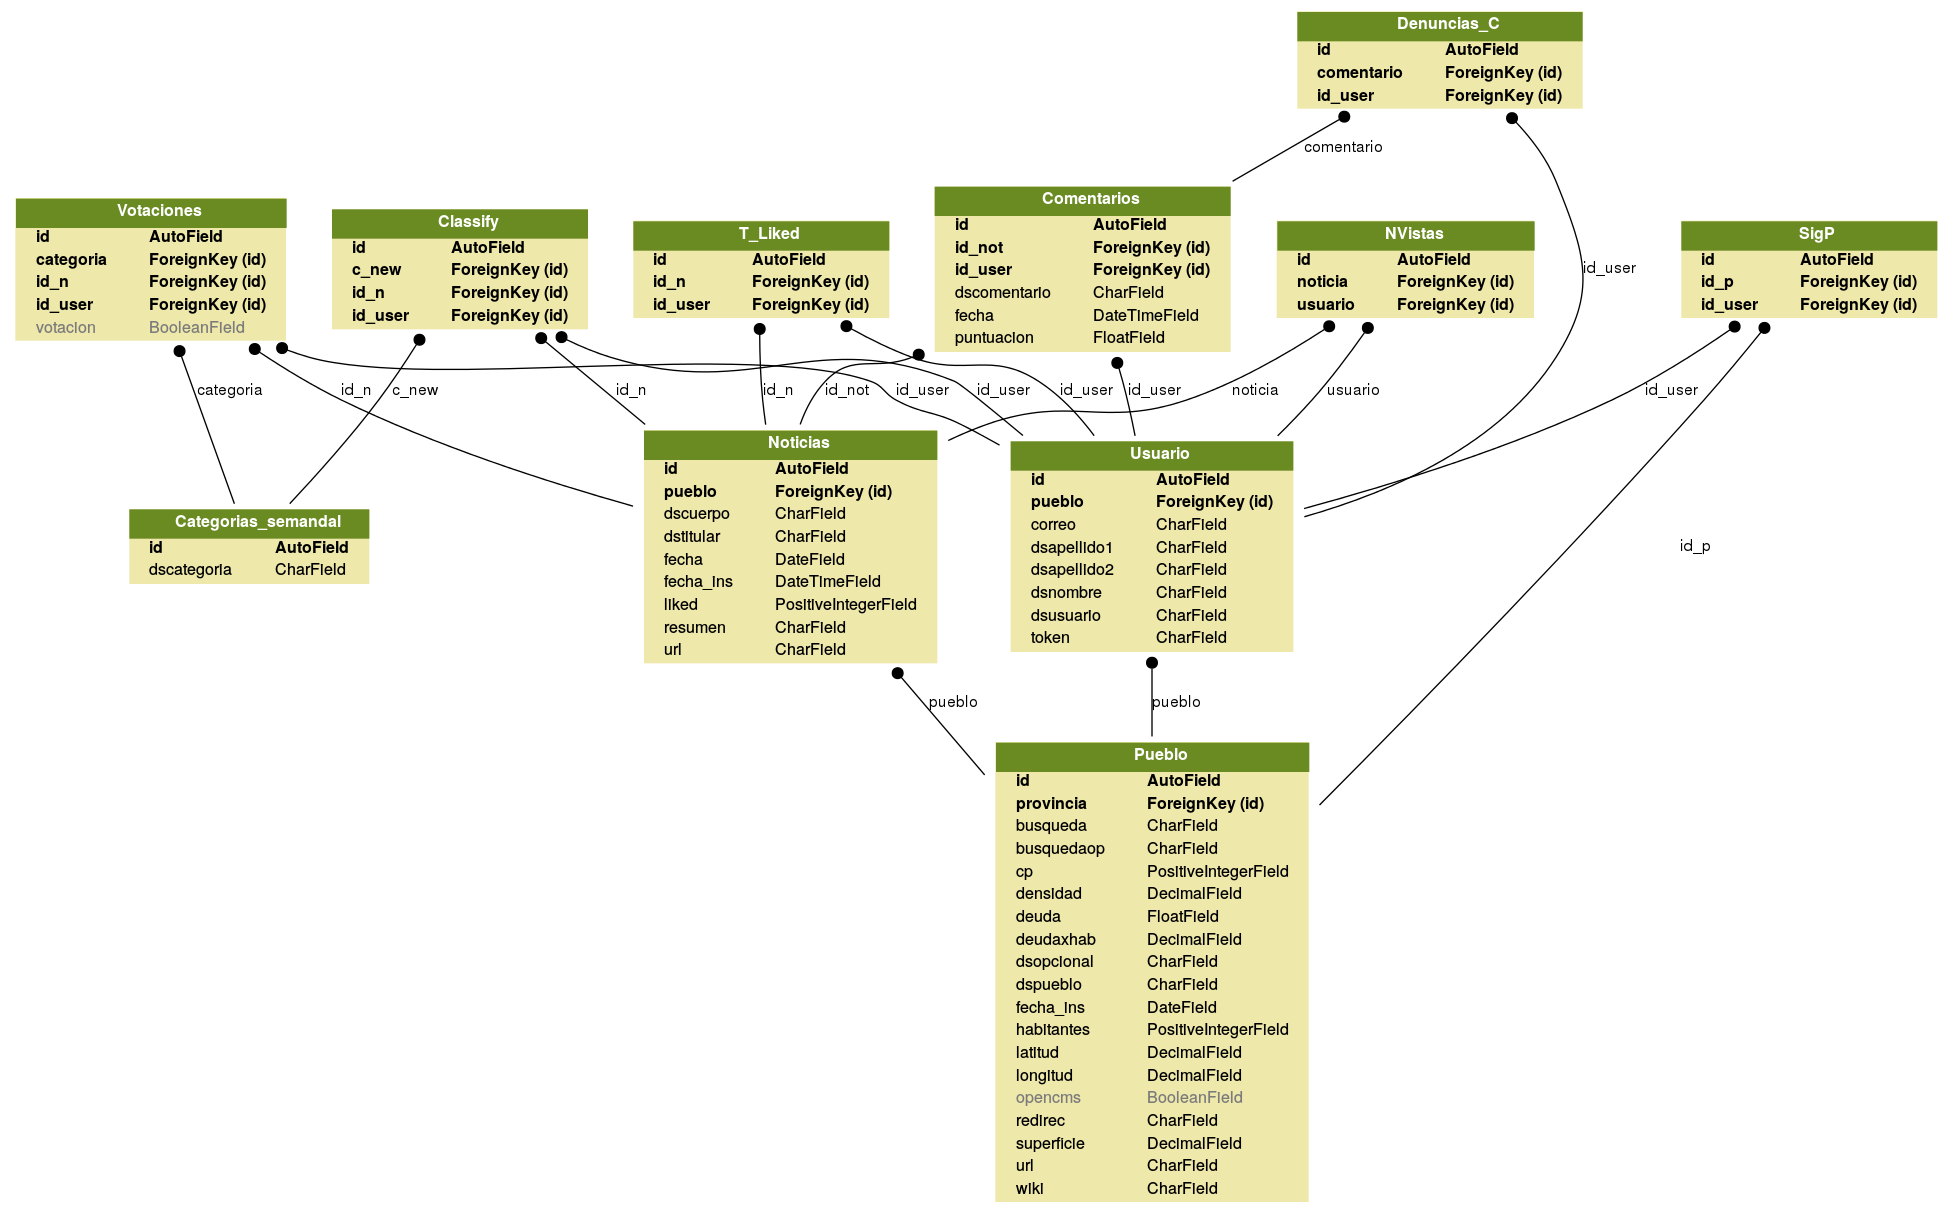
\includegraphics[scale=0.35]{basededatos/semandal_usuarios.png} 
\caption{Tablas de usuarios}
\label{fig:usuarios}
\end{center}
\end{sidewaysfigure}